% A point charge at rest and seen from a moving frame: E and B mix.
\documentclass[tikz,border=4pt]{standalone}
\usepackage{amsmath,amssymb}
\usetikzlibrary{arrows.meta,decorations.markings}
\definecolor{ecol}{HTML}{2F6DB5}\definecolor{bcol}{HTML}{D1552B}
\begin{document}
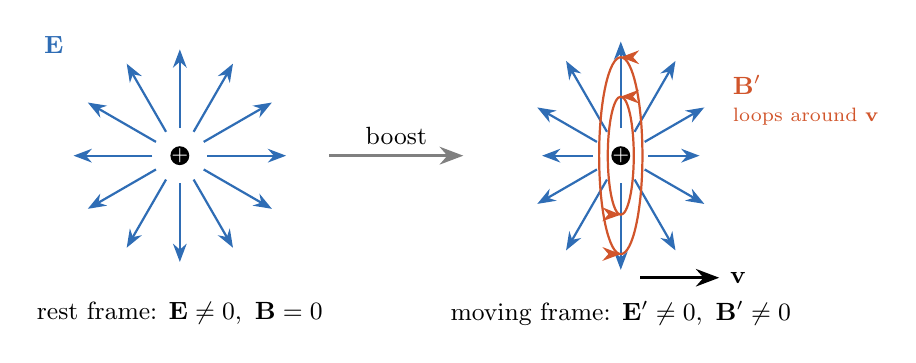
\begin{tikzpicture}[>=Stealth, every node/.style={font=\small}]
% rest frame
\begin{scope}
  \foreach \a in {0,30,...,330} \draw[ecol, thick, ->] (\a:0.35) -- (\a:1.35);
  \fill (0,0) circle (0.12) node[white, font=\scriptsize] {$+$};
  \node at (0,-2) {rest frame: $\mathbf E \neq 0,\ \mathbf B = 0$};
\end{scope}
% moving frame
\begin{scope}[xshift=5.6cm]
  \foreach \a in {0,30,...,330} {
    \pgfmathsetmacro{\r}{1.0+0.45*abs(sin(\a))}
    \draw[ecol, thick, ->] (\a:0.35) -- (\a:\r);
  }
  \foreach \rr in {0.75,1.25} {
    \draw[bcol, thick, postaction={decorate}, decoration={markings, mark=at position 0.25 with {\arrow{>}}, mark=at position 0.75 with {\arrow{>}}}]
      (0,0) ellipse ({0.22*\rr} and {\rr});
  }
  \fill (0,0) circle (0.12) node[white, font=\scriptsize] {$+$};
  \draw[very thick, ->] (0.25,-1.55) -- (1.25,-1.55) node[right] {$\mathbf v$};
  \node at (0,-2) {moving frame: $\mathbf E' \neq 0,\ \mathbf B' \neq 0$};
\end{scope}
\draw[gray, very thick, -{Stealth[length=3mm]}] (1.9,0) -- (3.6,0) node[midway, above, black] {boost};
\node[ecol] at (-1.6,1.4) {$\mathbf E$};
\node[bcol, anchor=west] at (6.9,0.9) {$\mathbf B'$};
\node[bcol, anchor=west, font=\scriptsize] at (6.9,0.5) {loops around $\mathbf v$};
\end{tikzpicture}
\end{document}
